\chapter{Week 5: Data-analyse in Python}

We hebben inmiddels een gedegen bassis kennis van \textit{Python} opgedaan gedurende dit vak. We hebben o.a. geleerd over loops, lijsten, functies en IO aansturing in \textit{Python}, en de vershillen gezien met \textit{C}. Een van de concepten die nog onbelicht is gebleven is het zogeheten 'object georiënteerd programmeren' (of \textit{OOP}).
Omdat dit een van de belangrijkste en handigste concepten van het programmeren is van de afgelopen decenia, én omdat we stiekem er toch al flink mee gewerkt hebben, gaan we in dit hoofdstuk ook dit thema belichten. Daarnaast gaan we deze week aan de slag met \textit{packages}, handige software bibliotheken die de functionaliteit van onze \textit{Python} omgeving kunnen uitbreiden. 

\section{Object georiënteerd programmeren}\index{Object georiënteerd programmeren}


\section{Packages}\index{Packages}
Een \textit{Package} in \textit{Python} is een verzameling van modules. Deze modules kunnen we weer in onze code gebruiken door deze te importeren met \pyth{import}. We hbben er in middel al een aantal van gebruikt bijv.: \pyth{math, time, gpiozero, RPi}, maar deze worden allemaal standaard meegeleverd. Je kunt ze ook heel eenvoudig zelf toevoegen aan je \textit{Python} omgeving, door gebruik te maken van \pyth{pip}. Dit programma kun je aanroepen vanaf de terminal:
\begin{lstlisting}[language=bash]
python3 -m pip install <naam_package>
\end{lstlisting}

\begin{remark}
Je hebt ongetwijfeld al een hele lijst geïnstalleerd zonder dat je het wist, je kunt het bekijken door het onderstaande in een terminal in te typen: 
\begin{lstlisting}[language=bash]
python3 -m pip list
\end{lstlisting}
En als je wat schijfruimte wilt vrij maken door packages te verwijderen die je niet langer gebruikt, kan dat met:
\begin{lstlisting}[language=bash]
python3 -m pip uninstall <naam_package>
\end{lstlisting}
\end{remark}

Om een beetje bekend te raken met \textit{pip}, gaan we als voorbeeld een kleine package installeren genaamd \pyth{camelcase}:
\begin{lstlisting}[language=bash]
python3 -m pip install camelcase
\end{lstlisting}

Probeer nu het volgende scriptje te draaien:
\begin{python}
from camelcase import CamelCase     # importeer onze nieuwe aanwinst

c = CamelCase()                     # Nodig om de package te kunnen gebruiken.
txt = 'pip onder de knie krijgen!'  # De tekst die omgezet dient te woren.

print(c.hump(txt))                  # Pas camelcase toe op de tekst.
\end{python}
Als dat lukt, is de module juist geïnstalleerd en heb je de basis van \textit{pip} onder de knie! (Deze packages worden overigens gedownload vanaf \url{https://pypi.org/}, kijk er gerust eens na en wellicht kom je er interressante tegen tussen de bijna 350.000 packages.) \\
Het aanpassen van hoofdletters is echter niet al te spannend, dus gaan we verder met een package waar we echt iets aan hebben: \textit{matplotlib}. 
\section{matplotlib}\index{matplotlib}

\begin{figure}[h!]
\centering
\includegraphics[scale=0.25]{Pictures/chapter07/matplotlib_logo.png}
% \caption{\small \textit{Matplotlib} logo. Bron: \url{https://matplotlib.org}}
\label{fig:mpllogo} % Unique label used for referencing the figure in-text
%\addcontentsline{toc}{figure}{Figure \ref{fig:webserver}} % Uncomment to add the figure to the table of contents
\end{figure}

Matplotlib is een verzameling aan tools voor het maken en bewerken van grafieken. 
\begin{exercise}
  Installeer Matplotlib
\end{exercise}

Om het te gebruiken in z'n meest simpele vorm zorg je ervoor dat je een reeks $x$-waardes hebt, en een reeks bijbehorende $y$-waardes. Deze kun je dan plotten (het daadwerkelijk tekenen van de grafiek) en de resulterende grafiek kun je tonen op het scherm:

\inputpython{code/chapter07/plot1.py}

Hieruit rolt grafiek \ref{fig:plot1} uit:
\begin{figure}[h!]
\centering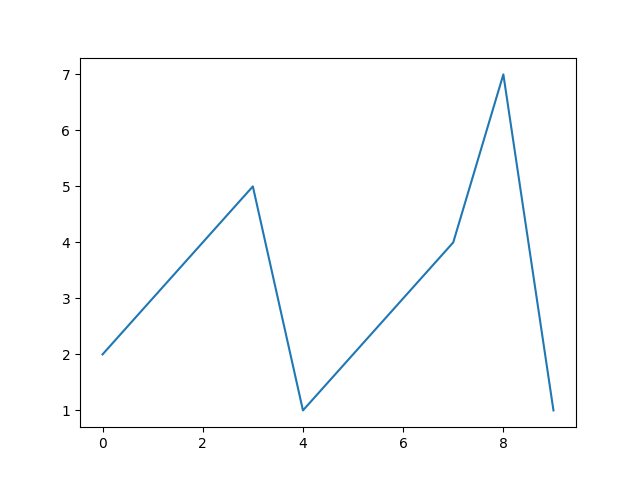
\includegraphics[scale=0.7]{Pictures/chapter07/plot1.png}
\caption{Simpele plot met \textit{Matplotlib}}
\label{fig:plot1} % Unique label used for referencing the figure in-text
%\addcontentsline{toc}{figure}{Figure \ref{fig:webserver}} % Uncomment to add the figure to the table of contents
\end{figure}

\begin{remark}
Kreeg je bij het runnen van bovenstaande code op de \textit{Pi} een error, in de trant van \textit{'Error retrieving accessibility bus address'}? Dan kan het zijn dat je een module in Linux mist, open een terminal en voer in: 
\begin{lstlisting}[language=bash]
sudo apt-get update
sudo apt-get install at-spi2-core
\end{lstlisting}
\end{remark}

Een grafiek is natuurlijk pas echt bruikbaar als deze netjes is opgemaakt met duidelijke labels voor de assen en eventueel een titel en een legenda. Ook dat is snel gepiept met \textit{matplotlib}. In het onderstaande stuk code voegen we dit toe aan ons eerdere script. Daarnaast is er een extra set met $y$-waardes toegevoegd, om $2$ verschillende meetmomenten na te bootsen.

\inputpython{code/chapter07/plot2.py}

De bonenstaande code produceert onderstaande grafiek \ref{fig:plot2}:
\begin{figure}[h!]
\centering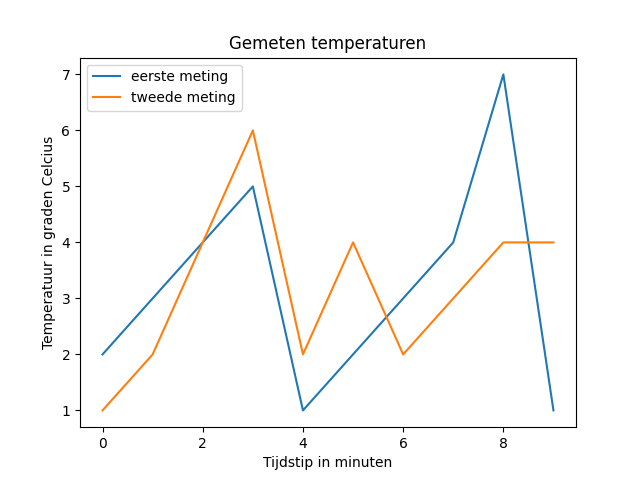
\includegraphics[scale=0.7]{Pictures/chapter07/plot2.png}
\caption{Uitgebreidere plot met \textit{Matplotlib}}
\label{fig:plot2} 
%\addcontentsline{toc}{figure}{Figure \ref{fig:webserver}} % Uncomment to add the figure to the table of contents
\end{figure}

\begin{exercise}
Zorg dat de eerste lijn rood gekleurd (\pyth{color}) wordt, en de tweede lijn groen en gestippeld (\pyth{linestyle}). \\
\textbf{TIP: } Gebruik hiervoor de documentatie van de packge op: \url{https://matplotlib.org}. 
\end{exercise}

\subsection{NumPy}\index{NumPy}

\begin{figure}[h!]
\centering
\includegraphics[scale=0.5]{Pictures/chapter07/numpy_logo.png}
% \caption{\small \textit{Matplotlib} logo. Bron: \url{https://matplotlib.org}}
\label{fig:numpylogo} % Unique label used for referencing the figure in-text
%\addcontentsline{toc}{figure}{Figure \ref{fig:webserver}} % Uncomment to add the figure to the table of contents
\end{figure}

De mogelijkheden van \textit{matplotlib} kunnen enorm uitgebreid worden in combinatie met andere packages. Een voor de hand liggende keuze daarin is bijvoorbeeld \textit{NumPy}. Die een enorm scala aan wiskundige tools met zich meebrengt. 

\begin{exercise}
Installeer NumPy 
\end{exercise}
We kunnen met de combinatie \textit{NumPy} en \textit{matplotlib} bijv. elke wiskunde functie die we kunnen bedenken op een makkelijke en overzichtelijke wijze plotten. Superhandig voor je wiskunde huiswerk ;). Als voorbeeldje volgt hieronder een klein scriptje die $y = sin(x)$ plot op een bereik van $-\pi$ tot $\pi$:
\inputpython{code/chapter07/plot_numpy.py}

De bonenstaande code produceert onderstaande grafiek \ref{fig:plot3}:
\begin{figure}[h!]
\centering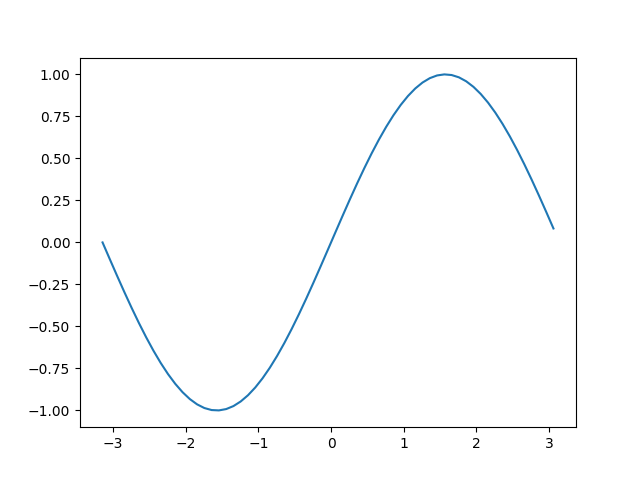
\includegraphics[scale=0.7]{Pictures/chapter07/sin.png}
\caption{Een sinus-functie tekenen met \textit{Matplotlib} en \textit{NumPy}.}
\label{fig:plot3} 
%\addcontentsline{toc}{figure}{Figure \ref{fig:webserver}} % Uncomment to add the figure to the table of contents
\end{figure}

Op regel $5$ wordt hier een reeks aan getallen gegenereerd door de \pyth{np.arange()}-functie. Valt je op dat deze functie nagenoeg hetzelfde eruit ziet (en werkt!) als de ingebouwde \pyth{range()}-functie? Het verschil zit 'm in dat \pyth{np.arange()} ook komma-getallen (floats) kan genereren. \\ 
Om een soortgelijke reden gebruiken we op regel $7$ \pyth{np.sin()} in plaats van \pyth{math.sin()}. De sinus functie uit \textit{NumPy} kan namelijk de sinus van een hele reeks getallen uitrekenen en dit weer teruggeven als een reeks getallen. De sinus-functie uit \pyth{math} kan enkel de sinus uitrekenen op $1$ getal per keer.
 
% \subsection{pip}\index{pip}

\section{Pandas}\index{Pandas}
\begin{figure}[h!]
\centering
\includegraphics[scale=0.2]{Pictures/chapter07/pandas_logo.png}
% \caption{\small \textit{Matplotlib} logo. Bron: \url{https://matplotlib.org}}
\label{fig:pandaslogo} % Unique label used for referencing the figure in-text
%\addcontentsline{toc}{figure}{Figure \ref{fig:webserver}} % Uncomment to add the figure to the table of contents
\end{figure}

% \subsection{Excel file edit}\index{Excel file edit}
Het tekenen van grafieken wordt een stuk intteressanter als je veel input data hebt. Die kun je bijvoorbeeld krijgen door een sensor periodiek te meten, maar ook door een spreadsheet in te laden. De package \textit{pandas} helpt je bij dat laatste enorm.

\begin{exercise}
Installeer de package \textit{Pandas} en z'n verschillende parser:
\begin{lstlisting}[language=bash]
python3 -m pip install pandas odfpy openpyxl xlrd
\end{lstlisting}
De laatste drie packages die hier worden geïnstalleerd zijn resp. nodig voor support van $.ods$- (LibreOffice), $.xslx$- (Microsoft Excel) en $.xls$- (Oude Microsoft Excel) bestanden. Mocht je bepaalde bestandsformaten niet gaan gebruiken, kun je die uiteraard overslaan.
\end{exercise}

Naast de \textit{Python} packages ben je natuurlijk ook een programma nodig dat spreadsheets kan maken en bewerken. Op je laptop gebruik je hier ongetwijfeld Microsoft Excel voor. Voor de Raspberry Pi moet je hier waarschijnlijk nog even een programma voor installeren. Voor een complete office suite variant, kun je bijv. LibreOffice installeren. Dit is een gratis, en een heel complete vervanger voor Microsoft Office (die overigens ook prima draait op je laptop ;) ).\\\\ 
Heb je nu geen zin in een grote download, kun je ook kiezen voor Gnumeric. Dat is gewoon een basic spreadsheet editor zonder poespas, maar wel met alle functionaliteit in huis die we tijdens dit vak nodig zijn.

\begin{exercise}
Installeer op basis van je voorkeur een spreadsheet programma op je Pi:
\begin{lstlisting}[language=bash]
sudo apt-get install libreoffce
\end{lstlisting}
of:
\begin{lstlisting}[language=bash]
sudo apt-get install gnumeric
\end{lstlisting}
\end{exercise}

Als voorbeeld heb ik de volgende spreadsheet aangemaakt: Een tabel met twee kolommen: 'Tijdstip' en 'Waarde', met elk $50$ rijen/waardes. 
\begin{figure}[h!]
\centering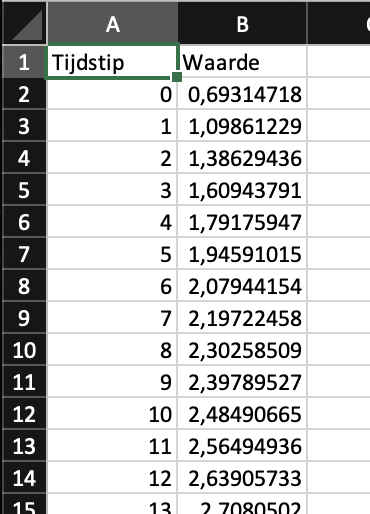
\includegraphics[scale=0.7]{Pictures/chapter07/excel1.png}
\caption{Voorbeeld spreadsheet gemaakt in Excel.}
\label{fig:excel1} % Unique label used for referencing the figure in-text
%\addcontentsline{toc}{figure}{Figure \ref{fig:webserver}} % Uncomment to add the figure to the table of contents
\end{figure}

Deze spreedsheet is dan met \textit{pandas} als volgt heel eenvoudig in te laden:
\inputpython{code/chapter07/exc1.py}

\begin{remark}
Heb je nu een spreadsheet met meerdere tabladen gemaakt en wil je een specifiek blad inladen met de naam 'Blad1'? Dat kan prima. Pas dan regel $5$ aan van de code naar: \\
\pyth{df = pd.read_excel('excel1.xlsx', sheet_name='Blad1')}
\end{remark}

Dit stukje code leest de $.xlsx$-bestand in, en print daarna alle namen van de kolommen op het scherm:
\begin{python}
Tijdstip
Waardes
\end{python}

Deze namen kunnen we daarna gebruiken om de daadwerkelijke data te benaderen en bijvoorbeeld te pringten met \textit{matplotlib}:

\inputpython{code/chapter07/exc2.py}

\newpage

Dit bovenstaande stukje code levert uiteindelijk de volgende grafiek op:

\begin{figure}[h!]
\centering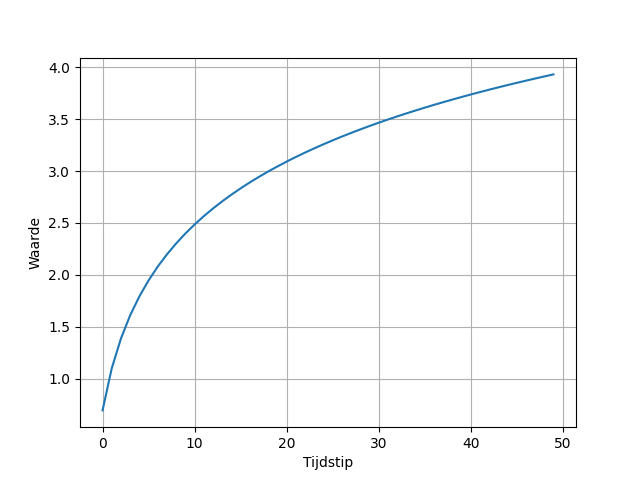
\includegraphics[scale=0.7]{Pictures/chapter07/plot3.png}
\caption{Plot gemaakt vanuit spreadsheet.}
\label{fig:plot3} % Unique label used for referencing the figure in-text
%\addcontentsline{toc}{figure}{Figure \ref{fig:webserver}} % Uncomment to add the figure to the table of contents
\end{figure}

\begin{remark}
Nerdy tip: Je kunt ook in plaats van zelf de x- en y-labels een naam te geven, dit af laten hangen van de gevonden kolomnamen:
\begin{python}
plt.xlabel(df.columns[0])
plt.ylabel(df.columns[1])
\end{python}
\end{remark}

Andersom kan natuurlijk ook: Je hebt data in je \textit{Python} script, en dat wil je opslaan als een spreadsheet. Dat is wat we met het volgende stukje code doen:

\inputpython{code/chapter07/toexc.py}

\newpage

Het gegenereerde bestand kunnen we openen met ons spreadsheet-programma, en zal er dan zo uitzien:

\begin{figure}[h!]
\centering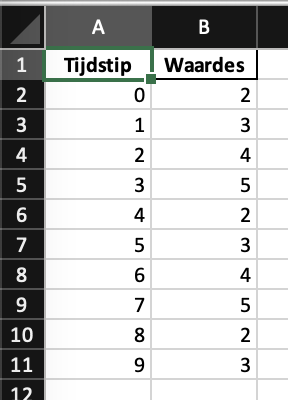
\includegraphics[scale=0.7]{Pictures/chapter07/excel2.png}
\caption{Spreadsheet gegenereerd vanuit \textit{Python}}
\label{fig:excel1} % Unique label used for referencing the figure in-text
%\addcontentsline{toc}{figure}{Figure \ref{fig:webserver}} % Uncomment to add the figure to the table of contents
\end{figure}

\begin{exercise}
Op regel $8$ gebruiken we de \pyth{zip()}-functie. Ga na in de interpreter wat deze functie precies doet met 2 lijsten. 
\end{exercise}

\newpage

\section{Opdrachten}\index{Opdrachten}
\begin{exercise}
Plot (in $1$ grafiek) met \textit{matplotlib} en \textit{NumPy} de functies: \\
$y_{1}=\sin(2\cdot x)$ en $y_{2}=4\cdot\cos(4\cdot x)$ tussen $-2\pi$ en $2\pi$.\\
Zorg ook voor een duidelijke legenda.
\end{exercise}

\begin{exercise}
\label{exc7:exc2}
Vraag van de gebruiker steeds een nummer, net zolang tot deze 'klaar' intypt. 
Voeg alle getallen die de gebruiker intypte steeds toe aan een lijst en print hier een nette grafiek van. (Begin voor de x-waardes te tellen bij $0$, en tel er steeds 1 bij op, voor elk ingevoerd getal).
\end{exercise}

\begin{exercise}
Breid het het programma van opdracht \ref{exc7:exc2} uit, zodat het programma ook een Excel sheet opslaat met alle ingevoerde cijfers.
\end{exercise}

\begin{exercise}
TODO: maak een klasse aan voor een RGB led op basis van RPi.GPIO en 3 verschillende leds
\end{exercise}

\begin{exercise}
$\\$
\end{exercise}

\begin{exercise}
$\\$
\end{exercise}

\begin{exercise}
$\\$
\end{exercise}

\begin{exercise}
$\\$
\end{exercise}

